\documentclass{article}

\usepackage{fancyhdr}
\usepackage{wrapfig}
\usepackage{extramarks}
\usepackage{multicol}
\usepackage{amsmath}
\usepackage{amsthm}
\usepackage{amsfonts}
\usepackage{tikz}
\usepackage[plain]{algorithm}
\usepackage{algpseudocode}
\usepackage{enumerate}
\usepackage[shortlabels]{enumitem}                                          
                    \setlist[enumerate, 1]{1\textsuperscript{o}}



\usepackage{listings}
\usepackage{xcolor}
\lstset { %
    language=C++,
    backgroundcolor=\color{black!5}, % set backgroundcolor
    basicstyle=\footnotesize,% basic font setting
}

%\usetikzlibrary{automata,positioning}
\usetikzlibrary{positioning,shapes,shadows,arrows,automata}

%
% Basic Document Settings
%

\topmargin=-0.45in
\evensidemargin=0in
\oddsidemargin=0in
\textwidth=6.5in
\textheight=9.0in
\headsep=0.25in

\linespread{1.1}

\pagestyle{fancy}
\lhead{\hmwkAuthorName}
\chead{\hmwkClass\ (\hmwkClassInstructor\ \hmwkClassTime): \hmwkTitle}
\rhead{\firstxmark}
\lfoot{\lastxmark}
\cfoot{\thepage}

\renewcommand\headrulewidth{0.4pt}
\renewcommand\footrulewidth{0.4pt}

\setlength\parindent{0pt}

%
% Create Problem Sections
%

\newcommand{\enterProblemHeader}[1]{
    \nobreak\extramarks{}{Problem \arabic{#1} continued on next page\ldots}\nobreak{}
    \nobreak\extramarks{Problem \arabic{#1} (continued)}{Problem \arabic{#1} continued on next page\ldots}\nobreak{}
}

\newcommand{\exitProblemHeader}[1]{
    \nobreak\extramarks{Problem \arabic{#1} (continued)}{Problem \arabic{#1} continued on next page\ldots}\nobreak{}
    \stepcounter{#1}
    \nobreak\extramarks{Problem \arabic{#1}}{}\nobreak{}
}

\setcounter{secnumdepth}{0}
\newcounter{partCounter}
\newcounter{homeworkProblemCounter}
\setcounter{homeworkProblemCounter}{1}
\nobreak\extramarks{Problem \arabic{homeworkProblemCounter}}{}\nobreak{}

%
% Homework Problem Environment
%
% This environment takes an optional argument. When given, it will adjust the
% problem counter. This is useful for when the problems given for your
% assignment aren't sequential. See the last 3 problems of this template for an
% example.
%
\newenvironment{homeworkProblem}[1][-1]{
    \ifnum#1>0
        \setcounter{homeworkProblemCounter}{#1}
    \fi
    \section{Problem \arabic{homeworkProblemCounter}}
    \setcounter{partCounter}{1}
    \enterProblemHeader{homeworkProblemCounter}
}{
    \exitProblemHeader{homeworkProblemCounter}
}

%
% Homework Details
%   - Title
%   - Due date
%   - Class
%   - Section/Time
%   - Instructor
%   - Author
%

\newcommand{\hmwkTitle}{Homework\ \#1}
\newcommand{\hmwkDueDate}{January 20 2015}
\newcommand{\hmwkClass}{CS581 Theory of Computation}
\newcommand{\hmwkClassTime}{Winter 2016}
\newcommand{\hmwkClassInstructor}{Harry H. Porter}
\newcommand{\hmwkAuthorName}{Konstantin Macarenco}

%
% Title Page
%

\title{
    \vspace{2in}
    \textmd{\textbf{\hmwkClass:\ \hmwkTitle}}\\
    \normalsize\vspace{0.1in}\small{Due\ on\ \hmwkDueDate\ at 2:00pm}\\
    \vspace{0.1in}\large{\textit{\hmwkClassInstructor\ \hmwkClassTime}}
    \vspace{3in}
}

\author{\textbf{\hmwkAuthorName}}
\date{}

\renewcommand{\part}[1]{\textbf{\large Part \Alph{partCounter}}\stepcounter{partCounter}\\}

%
% Various Helper Commands
%

% Useful for algorithms
\newcommand{\alg}[1]{\textsc{\bfseries \footnotesize #1}}

% For derivatives
\newcommand{\deriv}[1]{\frac{\mathrm{d}}{\mathrm{d}x} (#1)}

% For partial derivatives
\newcommand{\pderiv}[2]{\frac{\partial}{\partial #1} (#2)}

% Integral dx
\newcommand{\dx}{\mathrm{d}x}

% Alias for the Solution section header
\newcommand{\solution}{\textbf{\large Solution}}

% Probability commands: Expectation, Variance, Covariance, Bias
\newcommand{\E}{\mathrm{E}}
\newcommand{\Var}{\mathrm{Var}}
\newcommand{\Cov}{\mathrm{Cov}}
\newcommand{\Bias}{\mathrm{Bias}}

\begin{document}

\maketitle

\pagebreak

\begin{homeworkProblem}

\noindent

\begin{center}
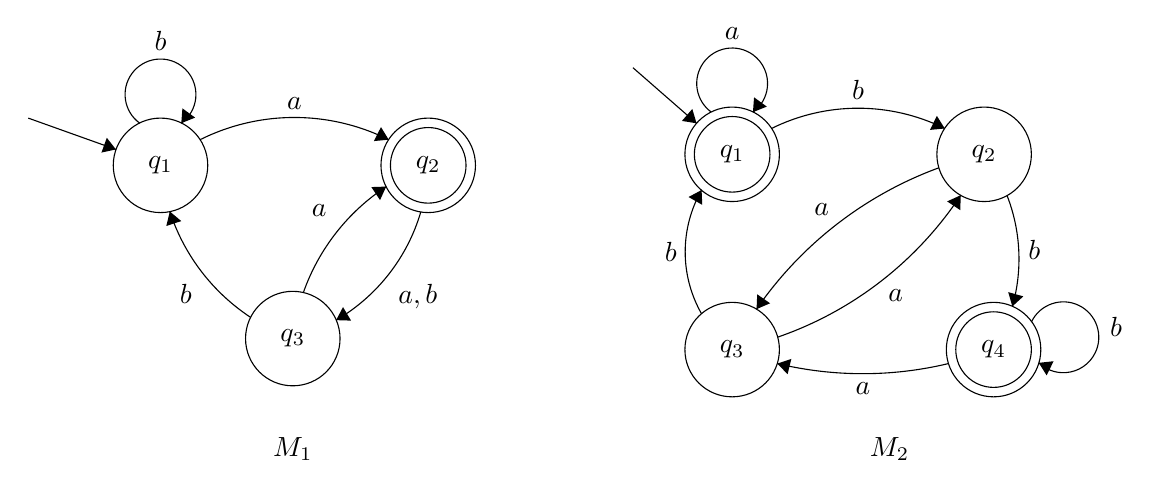
\begin{tikzpicture}[scale=0.2]
\tikzstyle{every node}+=[inner sep=0pt]
\draw [black] (9.8,-10.1) circle (3);
\draw (9.8,-10.1) node {$q_1$};
\draw [black] (26.8,-10.1) circle (3);
\draw (26.8,-10.1) node {$q_2$};
\draw [black] (26.8,-10.1) circle (2.4);
\draw [black] (18.2,-21.1) circle (3);
\draw (18.2,-21.1) node {$q_3$};
\draw (18.2,-28.1) node {$M_1$};
\draw [black] (46.1,-9.4) circle (3);
\draw (46.1,-9.4) node {$q_1$};
\draw [black] (46.1,-9.4) circle (2.4);
\draw [black] (62.1,-9.4) circle (3);
\draw (62.1,-9.4) node {$q_2$};
\draw [black] (46.1,-21.8) circle (3);
\draw (46.1,-21.8) node {$q_3$};
\draw (56.1,-28.1) node {$M_2$};
\draw [black] (62.7,-21.8) circle (3);
\draw (62.7,-21.8) node {$q_4$};
\draw [black] (62.7,-21.8) circle (2.4);
\draw [black] (8.477,-7.42) arc (234:-54:2.25);
\draw (9.8,-2.85) node [above] {$b$};
\fill [black] (11.12,-7.42) -- (12,-7.07) -- (11.19,-6.48);
\draw [black] (12.312,-8.472) arc (116.53845:63.46155:13.402);
\fill [black] (24.29,-8.47) -- (23.8,-7.67) -- (23.35,-8.56);
\draw (18.3,-6.56) node [above] {$a$};
\draw [black] (26.329,-13.055) arc (-16.32928:-59.70861:11.807);
\fill [black] (20.95,-19.93) -- (21.9,-19.96) -- (21.39,-19.1);
\draw (24.87,-18.42) node [right] {$a,b$};
\draw [black] (18.87,-18.182) arc (160.62375:123.33837:13.357);
\fill [black] (24.13,-11.45) -- (23.19,-11.48) -- (23.74,-12.31);
\draw (20.38,-12.97) node [left] {$a$};
\draw [black] (15.525,-19.756) arc (-123.37352:-161.89315:12.821);
\fill [black] (10.39,-13.03) -- (10.17,-13.95) -- (11.12,-13.64);
\draw (11.82,-18.24) node [left] {$b$};
\draw [black] (1.4,-7.1) -- (6.97,-9.09);
\fill [black] (6.97,-9.09) -- (6.39,-8.35) -- (6.05,-9.29);
\draw [black] (39.8,-3.9) -- (43.84,-7.43);
\fill [black] (43.84,-7.43) -- (43.57,-6.52) -- (42.91,-7.28);
\draw [black] (44.777,-6.72) arc (234:-54:2.25);
\draw (46.1,-2.15) node [above] {$a$};
\fill [black] (47.42,-6.72) -- (48.3,-6.37) -- (47.49,-5.78);
\draw [black] (48.602,-7.758) arc (116.33712:63.66288:12.392);
\fill [black] (59.6,-7.76) -- (59.1,-6.96) -- (58.66,-7.85);
\draw (54.1,-5.97) node [above] {$b$};
\draw [black] (63.554,-12.014) arc (21.33103:-15.7906:11.079);
\fill [black] (63.89,-19.06) -- (64.59,-18.42) -- (63.63,-18.15);
\draw (64.87,-15.49) node [right] {$b$};
\draw [black] (65.109,-20.032) arc (154.00798:-133.99202:2.25);
\draw (70.07,-20.37) node [right] {$b$};
\fill [black] (65.57,-22.64) -- (66.07,-23.44) -- (66.51,-22.54);
\draw [black] (59.836,-22.687) arc (-76.49247:-103.50753:23.274);
\fill [black] (48.96,-22.69) -- (49.62,-23.36) -- (49.86,-22.39);
\draw (54.4,-23.83) node [below] {$a$};
\draw [black] (60.612,-12.003) arc (-33.50518:-70.94346:22.905);
\fill [black] (60.61,-12) -- (59.75,-12.39) -- (60.59,-12.95);
\draw (56.49,-17.96) node [below] {$a$};
\draw [black] (47.646,-19.231) arc (145.41007:110.14129:24.182);
\fill [black] (47.65,-19.23) -- (48.51,-18.86) -- (47.69,-18.29);
\draw (51.79,-13.35) node [above] {$a$};
\draw [black] (44.161,-19.534) arc (-150.27637:-209.72363:7.935);
\fill [black] (44.16,-11.67) -- (43.33,-12.11) -- (44.2,-12.61);
\draw (42.62,-15.6) node [left] {$b$};
\end{tikzpicture}
\end{center}

\hspace{1cm}
\begin{enumerate}[a., leftmargin = 0.5cm, nosep]
\itemsep0em
\item Start State: $M_1$ - $q_1$, $M_2$ - $q_1$
\item Set of accept states $M_1$ - $F=\{q_2\}$, $M_2$ - $F=\{q_1,q_4\}$, 
\item $M_1$ = $\{q_1,q_2,q_3,q_1,q_1\}$, $M_2$ $=\{q_1,q_1,q_1,q_2,q_4\}$
\item $M_1$ No, $M_2$ Yes
\item $M_1$ No, $M_2$ Yes
\end{enumerate}
\end{homeworkProblem}

\begin{homeworkProblem}
$M_1$
\begin{enumerate}[1., leftmargin = 0.5cm]
\itemsep0em
\item $Q = \{q_1,q_2,q_3\}$
\item $\sum = \{a,b\}$
\item $\delta$ described as
\begin{table}[h!]
\centering
\caption{$M_1$ Transition function}
\label{my-label}
\begin{tabular}{l|ll}
      & a     &    b  \\ \hline
$q_1$ & $q_2$ & $q_1$ \\
$q_2$ & $q_3$ & $q_3$ \\
$q_3$ & $q_2$ & $q_1$
\end{tabular}
\end{table}
\item Start state $q_1 \in Q$
\item $F = \{q_3\} \subseteq Q$ Start state $q_1 \in Q$
\end{enumerate}
\pagebreak
$M_2$
\begin{enumerate}[1., leftmargin = 0.5cm]
\itemsep0em
\item $Q = \{q_1,q_2,q_3,q_4\}$
\item $\sum = \{a,b\}$
\item $\delta$ described as
\begin{table}[h!]
\centering
\caption{$M_2$ Transition function}
\label{my-label}
\begin{tabular}{l|ll}
      & a     &    b  \\ \hline
$q_1$ & $q_1$ & $q_2$ \\
$q_2$ & $q_3$ & $q_4$ \\
$q_3$ & $q_2$ & $q_1$ \\
$q_4$ & $q_3$ & $q_4$
\end{tabular}
\end{table}
\item Start state $q_1 \in Q$
\item $F = \{q_1,q_4\} \subseteq Q$ Start state $q_1 \in Q$
\end{enumerate}

\end{homeworkProblem}

\begin{homeworkProblem}

\begin{center}
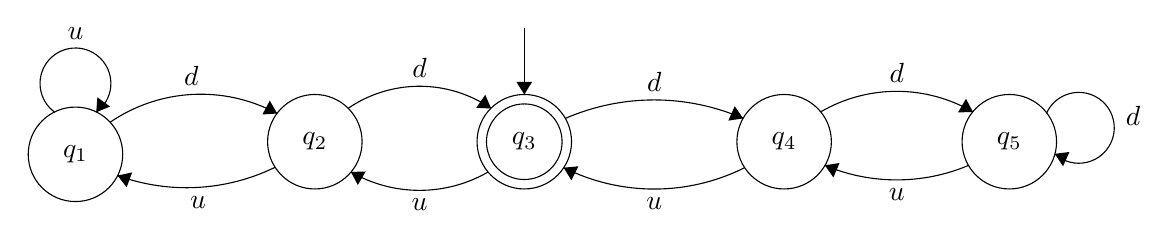
\begin{tikzpicture}[scale=0.2]
\tikzstyle{every node}+=[inner sep=0pt]
\draw [black] (8.3,-10.1) circle (3);
\draw (8.3,-10.1) node {$q_1$};
\draw [black] (23.5,-9.3) circle (3);
\draw (23.5,-9.3) node {$q_2$};
\draw [black] (36.8,-9.3) circle (3);
\draw (36.8,-9.3) node {$q_3$};
\draw [black] (36.8,-9.3) circle (2.4);
\draw [black] (53.3,-9.3) circle (3);
\draw (53.3,-9.3) node {$q_4$};
\draw [black] (67.6,-9.3) circle (3);
\draw (67.6,-9.3) node {$q_5$};
\draw [black] (36.8,-2.1) -- (36.8,-6.3);
\fill [black] (36.8,-6.3) -- (37.3,-5.5) -- (36.3,-5.5);
\draw [black] (6.977,-7.42) arc (234:-54:2.25);
\draw (8.3,-2.85) node [above] {$u$};
\fill [black] (9.62,-7.42) -- (10.5,-7.07) -- (9.69,-6.48);
\draw [black] (10.492,-8.068) arc (124.40866:61.61691:10.202);
\fill [black] (21.11,-7.51) -- (20.64,-6.69) -- (20.17,-7.57);
\draw (15.66,-5.75) node [above] {$d$};
\draw [black] (20.983,-10.92) arc (-63.94561:-110.02881:12.805);
\fill [black] (10.97,-11.45) -- (11.55,-12.19) -- (11.9,-11.25);
\draw (16.09,-12.75) node [below] {$u$};
\draw [black] (25.604,-7.186) arc (124.43892:55.56108:8.038);
\fill [black] (34.7,-7.19) -- (34.32,-6.32) -- (33.75,-7.15);
\draw (30.15,-5.28) node [above] {$d$};
\draw [black] (34.512,-11.217) arc (-59.92561:-120.07439:8.703);
\fill [black] (25.79,-11.22) -- (26.23,-12.05) -- (26.73,-11.19);
\draw (30.15,-12.89) node [below] {$u$};
\draw [black] (39.404,-7.821) arc (113.51604:66.48396:14.15);
\fill [black] (50.7,-7.82) -- (50.16,-7.04) -- (49.76,-7.96);
\draw (45.05,-6.15) node [above] {$d$};
\draw [black] (50.8,-10.945) arc (-63.35828:-116.64172:12.822);
\fill [black] (39.3,-10.95) -- (39.79,-11.75) -- (40.24,-10.86);
\draw (45.05,-12.81) node [below] {$u$};
\draw [black] (55.613,-7.409) arc (120.29559:59.70441:9.588);
\fill [black] (65.29,-7.41) -- (64.85,-6.57) -- (64.34,-7.44);
\draw (60.45,-5.6) node [above] {$d$};
\draw [black] (65.013,-10.803) arc (-67.15252:-112.84748:11.752);
\fill [black] (55.89,-10.8) -- (56.43,-11.57) -- (56.82,-10.65);
\draw (60.45,-12.23) node [below] {$u$};
\draw [black] (69.968,-7.478) arc (155.30993:-132.69007:2.25);
\draw (74.96,-7.66) node [right] {$d$};
\fill [black] (70.49,-10.07) -- (71.01,-10.86) -- (71.42,-9.95);
\end{tikzpicture}
\end{center}
\end{homeworkProblem}


\begin{homeworkProblem}
\textbf{a}
\begin{center}
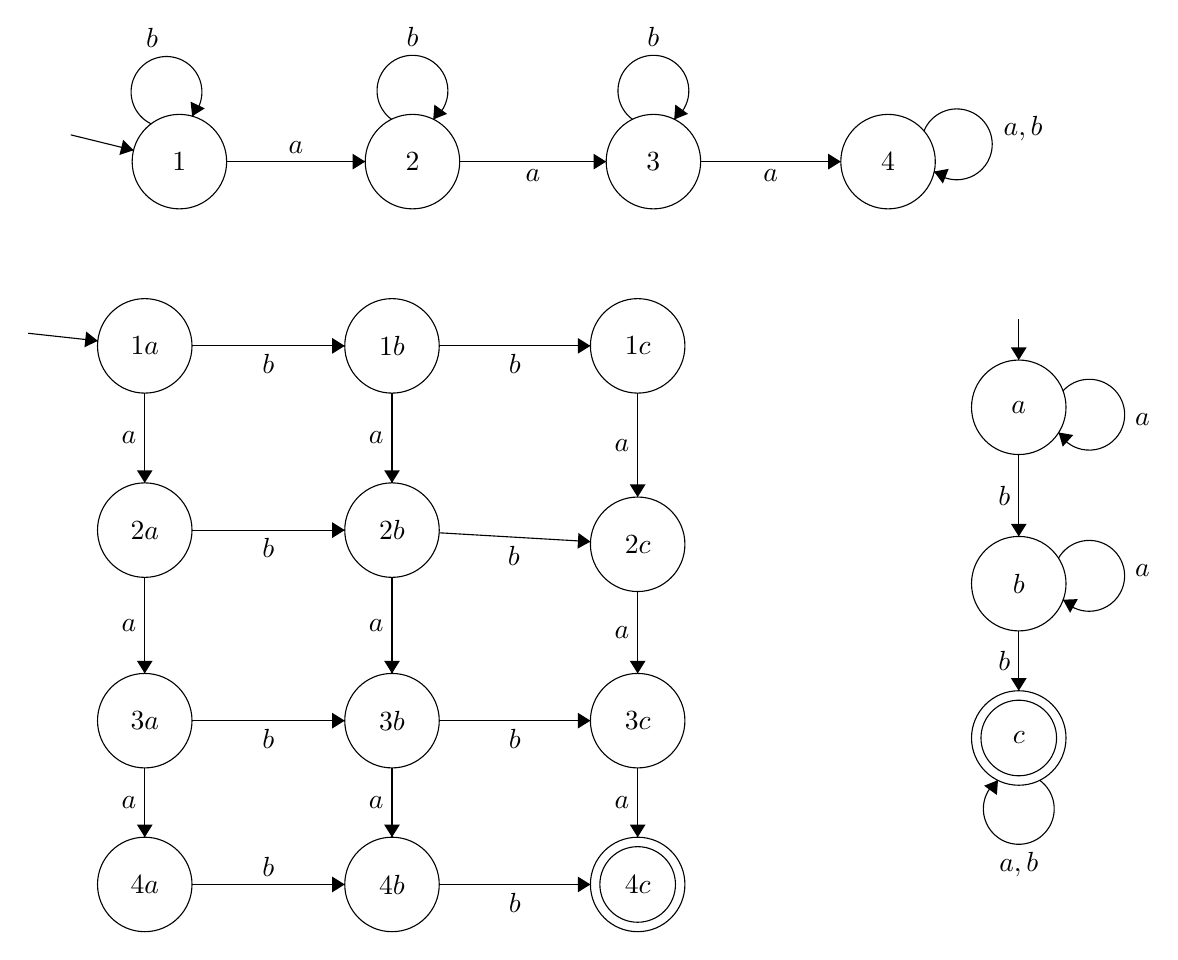
\begin{tikzpicture}[scale=0.2]
\tikzstyle{every node}+=[inner sep=0pt]
\draw [black] (6.9,-21) circle (3);
\draw (6.9,-21) node {$1a$};
\draw [black] (22.6,-21) circle (3);
\draw (22.6,-21) node {$1b$};
\draw [black] (38.2,-21) circle (3);
\draw (38.2,-21) node {$1c$};
\draw [black] (6.9,-32.7) circle (3);
\draw (6.9,-32.7) node {$2a$};
\draw [black] (22.6,-32.7) circle (3);
\draw (22.6,-32.7) node {$2b$};
\draw [black] (38.2,-33.6) circle (3);
\draw (38.2,-33.6) node {$2c$};
\draw [black] (6.9,-44.8) circle (3);
\draw (6.9,-44.8) node {$3a$};
\draw [black] (22.6,-44.8) circle (3);
\draw (22.6,-44.8) node {$3b$};
\draw [black] (38.2,-44.8) circle (3);
\draw (38.2,-44.8) node {$3c$};
\draw [black] (6.9,-55.2) circle (3);
\draw (6.9,-55.2) node {$4a$};
\draw [black] (22.6,-55.2) circle (3);
\draw (22.6,-55.2) node {$4b$};
\draw [black] (38.2,-55.2) circle (3);
\draw (38.2,-55.2) node {$4c$};
\draw [black] (38.2,-55.2) circle (2.4);
\draw [black] (9.1,-9.3) circle (3);
\draw (9.1,-9.3) node {$1$};
\draw [black] (23.9,-9.3) circle (3);
\draw (23.9,-9.3) node {$2$};
\draw [black] (39.2,-9.3) circle (3);
\draw (39.2,-9.3) node {$3$};
\draw [black] (54.1,-9.3) circle (3);
\draw (54.1,-9.3) node {$4$};
\draw [black] (62.4,-24.9) circle (3);
\draw (62.4,-24.9) node {$a$};
\draw [black] (62.4,-36.1) circle (3);
\draw (62.4,-36.1) node {$b$};
\draw [black] (62.4,-45.9) circle (3);
\draw (62.4,-45.9) node {$c$};
\draw [black] (62.4,-45.9) circle (2.4);
\draw [black] (9.9,-21) -- (19.6,-21);
\fill [black] (19.6,-21) -- (18.8,-20.5) -- (18.8,-21.5);
\draw (14.75,-21.5) node [below] {$b$};
\draw [black] (25.6,-21) -- (35.2,-21);
\fill [black] (35.2,-21) -- (34.4,-20.5) -- (34.4,-21.5);
\draw (30.4,-21.5) node [below] {$b$};
\draw [black] (9.9,-32.7) -- (19.6,-32.7);
\fill [black] (19.6,-32.7) -- (18.8,-32.2) -- (18.8,-33.2);
\draw (14.75,-33.2) node [below] {$b$};
\draw [black] (25.6,-32.87) -- (35.2,-33.43);
\fill [black] (35.2,-33.43) -- (34.44,-32.88) -- (34.38,-33.88);
\draw (30.33,-33.7) node [below] {$b$};
\draw [black] (9.9,-44.8) -- (19.6,-44.8);
\fill [black] (19.6,-44.8) -- (18.8,-44.3) -- (18.8,-45.3);
\draw (14.75,-45.3) node [below] {$b$};
\draw [black] (25.6,-44.8) -- (35.2,-44.8);
\fill [black] (35.2,-44.8) -- (34.4,-44.3) -- (34.4,-45.3);
\draw (30.4,-45.3) node [below] {$b$};
\draw [black] (9.9,-55.2) -- (19.6,-55.2);
\fill [black] (19.6,-55.2) -- (18.8,-54.7) -- (18.8,-55.7);
\draw (14.75,-54.7) node [above] {$b$};
\draw [black] (25.6,-55.2) -- (35.2,-55.2);
\fill [black] (35.2,-55.2) -- (34.4,-54.7) -- (34.4,-55.7);
\draw (30.4,-55.7) node [below] {$b$};
\draw [black] (6.9,-24) -- (6.9,-29.7);
\fill [black] (6.9,-29.7) -- (7.4,-28.9) -- (6.4,-28.9);
\draw (6.4,-26.85) node [left] {$a$};
\draw [black] (22.6,-24) -- (22.6,-29.7);
\fill [black] (22.6,-29.7) -- (23.1,-28.9) -- (22.1,-28.9);
\draw (22.1,-26.85) node [left] {$a$};
\draw [black] (38.2,-24) -- (38.2,-30.6);
\fill [black] (38.2,-30.6) -- (38.7,-29.8) -- (37.7,-29.8);
\draw (37.7,-27.3) node [left] {$a$};
\draw [black] (6.9,-35.7) -- (6.9,-41.8);
\fill [black] (6.9,-41.8) -- (7.4,-41) -- (6.4,-41);
\draw (6.4,-38.75) node [left] {$a$};
\draw [black] (22.6,-35.7) -- (22.6,-41.8);
\fill [black] (22.6,-41.8) -- (23.1,-41) -- (22.1,-41);
\draw (22.1,-38.75) node [left] {$a$};
\draw [black] (38.2,-36.6) -- (38.2,-41.8);
\fill [black] (38.2,-41.8) -- (38.7,-41) -- (37.7,-41);
\draw (37.7,-39.2) node [left] {$a$};
\draw [black] (6.9,-47.8) -- (6.9,-52.2);
\fill [black] (6.9,-52.2) -- (7.4,-51.4) -- (6.4,-51.4);
\draw (6.4,-50) node [left] {$a$};
\draw [black] (22.6,-47.8) -- (22.6,-52.2);
\fill [black] (22.6,-52.2) -- (23.1,-51.4) -- (22.1,-51.4);
\draw (22.1,-50) node [left] {$a$};
\draw [black] (38.2,-47.8) -- (38.2,-52.2);
\fill [black] (38.2,-52.2) -- (38.7,-51.4) -- (37.7,-51.4);
\draw (37.7,-50) node [left] {$a$};
\draw [black] (-0.5,-20.2) -- (3.92,-20.68);
\fill [black] (3.92,-20.68) -- (3.18,-20.09) -- (3.07,-21.09);
\draw [black] (12.1,-9.3) -- (20.9,-9.3);
\fill [black] (20.9,-9.3) -- (20.1,-8.8) -- (20.1,-9.8);
\draw (16.5,-8.8) node [above] {$a$};
\draw [black] (26.9,-9.3) -- (36.2,-9.3);
\fill [black] (36.2,-9.3) -- (35.4,-8.8) -- (35.4,-9.8);
\draw (31.55,-9.8) node [below] {$a$};
\draw [black] (42.2,-9.3) -- (51.1,-9.3);
\fill [black] (51.1,-9.3) -- (50.3,-8.8) -- (50.3,-9.8);
\draw (46.65,-9.8) node [below] {$a$};
\draw [black] (56.377,-7.364) arc (158.10808:-129.89192:2.25);
\draw (61.41,-7.19) node [right] {$a,b$};
\fill [black] (57.02,-9.93) -- (57.58,-10.69) -- (57.95,-9.76);
\draw [black] (37.877,-6.62) arc (234:-54:2.25);
\draw (39.2,-2.05) node [above] {$b$};
\fill [black] (40.52,-6.62) -- (41.4,-6.27) -- (40.59,-5.68);
\draw [black] (22.577,-6.62) arc (234:-54:2.25);
\draw (23.9,-2.05) node [above] {$b$};
\fill [black] (25.22,-6.62) -- (26.1,-6.27) -- (25.29,-5.68);
\draw [black] (7.312,-6.906) arc (244.49148:-43.50852:2.25);
\draw (7.36,-2.07) node [above] {$b$};
\fill [black] (9.91,-6.42) -- (10.71,-5.92) -- (9.81,-5.49);
\draw [black] (2.2,-7.6) -- (6.19,-8.58);
\fill [black] (6.19,-8.58) -- (5.53,-7.91) -- (5.29,-8.88);
\draw [black] (62.4,-19.3) -- (62.4,-21.9);
\fill [black] (62.4,-21.9) -- (62.9,-21.1) -- (61.9,-21.1);
\draw [black] (62.4,-27.9) -- (62.4,-33.1);
\fill [black] (62.4,-33.1) -- (62.9,-32.3) -- (61.9,-32.3);
\draw (61.9,-30.5) node [left] {$b$};
\draw [black] (62.4,-39.1) -- (62.4,-42.9);
\fill [black] (62.4,-42.9) -- (62.9,-42.1) -- (61.9,-42.1);
\draw (61.9,-41) node [left] {$b$};
\draw [black] (63.723,-48.58) arc (54:-234:2.25);
\draw (62.4,-53.15) node [below] {$a,b$};
\fill [black] (61.08,-48.58) -- (60.2,-48.93) -- (61.01,-49.52);
\draw [black] (65.203,-23.865) arc (137.99099:-150.00901:2.25);
\draw (69.76,-25.7) node [right] {$a$};
\fill [black] (64.93,-26.5) -- (65.19,-27.4) -- (65.86,-26.66);
\draw [black] (64.917,-34.49) arc (150.34019:-137.65981:2.25);
\draw (69.76,-35.25) node [right] {$a$};
\fill [black] (65.21,-37.12) -- (65.66,-37.95) -- (66.15,-37.08);
\end{tikzpicture}
\end{center}

\end{homeworkProblem}
\end{document}
